%mark = star, diamond, square, otimes
%\documentclass{article}
%\usepackage{pgfplots}
%\usepackage[justification=centering]{caption}
%\pgfplotsset{compat=newest}
%\begin{document}
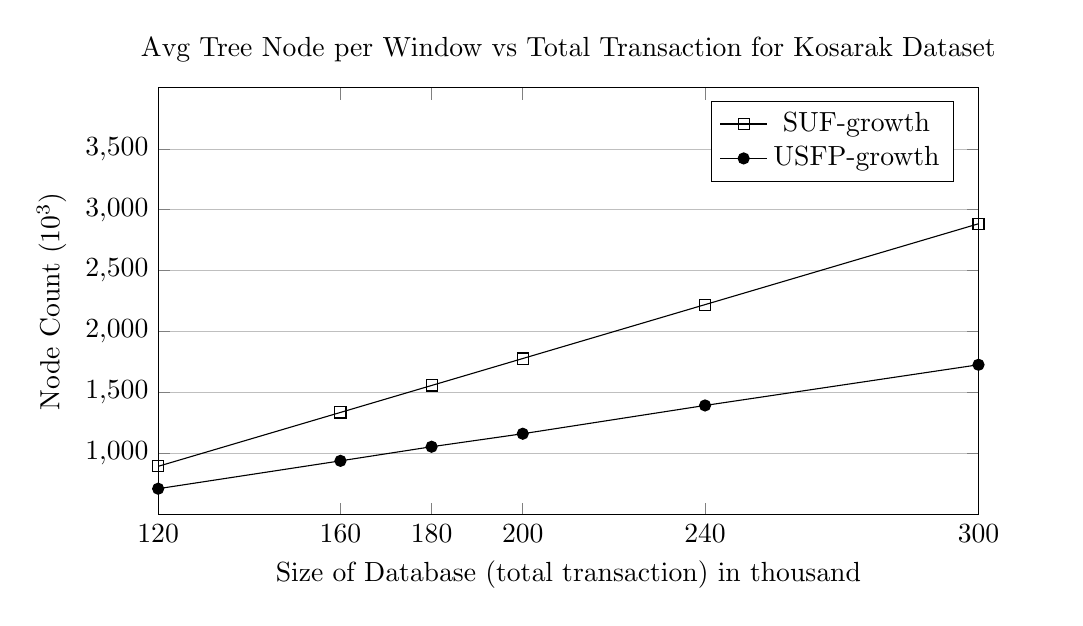
\begin{tikzpicture}
\begin{axis}[
	title={\parbox{\linewidth}{\centering Avg Tree Node per Window vs Total Transaction for Kosarak Dataset}},
	width=12cm,
	height=7cm,
    xlabel={Size of Database (total transaction) in thousand},
    ylabel={Node Count ($10^3$)},
    xmin=120, xmax=300,
    ymin=500, ymax=4000,
    xtick={120,160,180,200,240,300},
    ytick={1000,1500,2000,2500,3000,3500},
    legend pos=north east,
    ymajorgrids=true,
    grid style={line width=.2pt,draw=gray!50},
]
 
\addplot[
    solid, every mark/.append style={solid, fill=gray}, mark=square
    ]
    coordinates {
			(120,	895.299)
			(160,	1337.507)
			(180,	1558.611)
			(200,	1779.715)
			(240,	2221.923)
			(300,	2885.235)

	};
    \addlegendentry{SUF-growth}
\addplot[
    solid, every mark/.append style={solid, fill=black}, mark=*
    ]
    coordinates {
			(120,	711.772)
			(160,	940.241)
			(180,	1056.093)
			(200,	1162.692)
			(240,	1394.691)
			(300,	1728.543)


};
    \addlegendentry{USFP-growth}
 
\end{axis}
\end{tikzpicture}
%\end{document}